% Graphic for TeX using PGF
% Title: /home/attila/work/DesignPatterns/arm/ObjFact.dia
% Creator: Dia v0.97.2
% CreationDate: Fri Mar  7 22:13:09 2014
% For: attila
% \usepackage{tikz}
% The following commands are not supported in PSTricks at present
% We define them conditionally, so when they are implemented,
% this pgf file will use them.
\ifx\du\undefined
  \newlength{\du}
\fi
\setlength{\du}{15\unitlength}
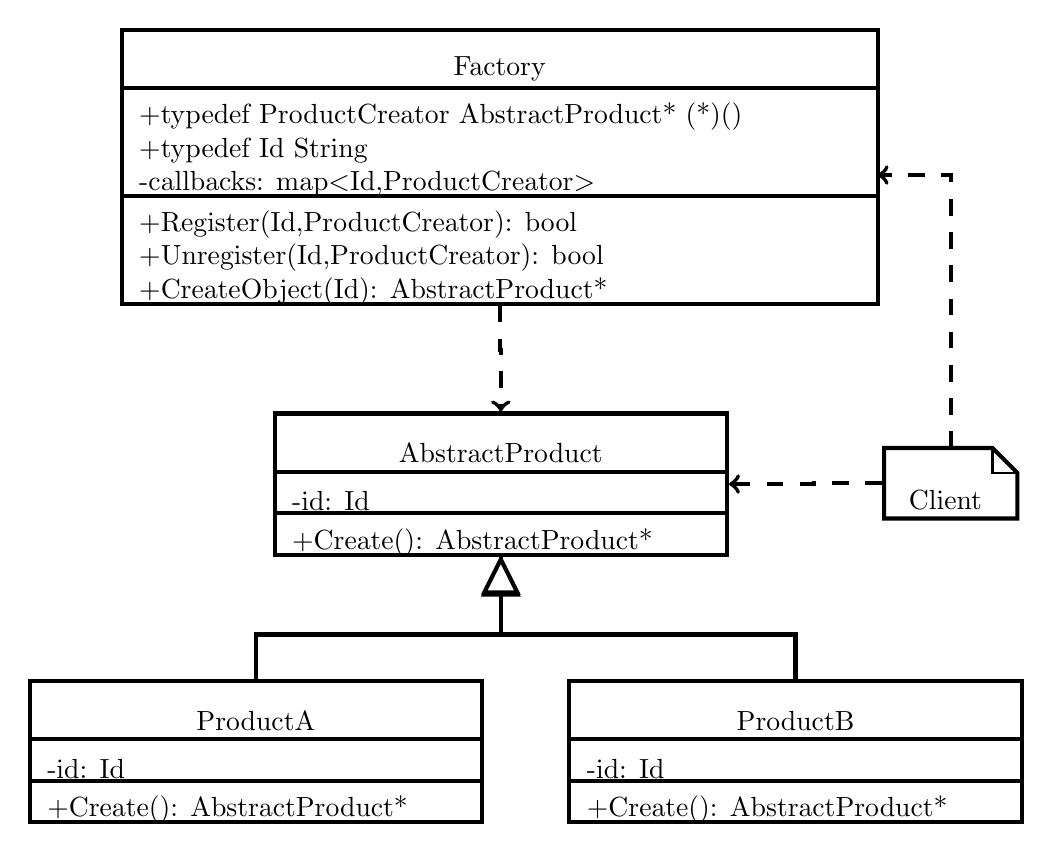
\begin{tikzpicture}
\pgftransformxscale{1.000000}
\pgftransformyscale{-1.000000}
\definecolor{dialinecolor}{rgb}{0.000000, 0.000000, 0.000000}
\pgfsetstrokecolor{dialinecolor}
\definecolor{dialinecolor}{rgb}{1.000000, 1.000000, 1.000000}
\pgfsetfillcolor{dialinecolor}
\pgfsetlinewidth{0.100000\du}
\pgfsetdash{}{0pt}
\definecolor{dialinecolor}{rgb}{1.000000, 1.000000, 1.000000}
\pgfsetfillcolor{dialinecolor}
\fill (27.315300\du,-4.194410\du)--(27.315300\du,-2.794410\du)--(45.525300\du,-2.794410\du)--(45.525300\du,-4.194410\du)--cycle;
\definecolor{dialinecolor}{rgb}{0.000000, 0.000000, 0.000000}
\pgfsetstrokecolor{dialinecolor}
\draw (27.315300\du,-4.194410\du)--(27.315300\du,-2.794410\du)--(45.525300\du,-2.794410\du)--(45.525300\du,-4.194410\du)--cycle;
% setfont left to latex
\definecolor{dialinecolor}{rgb}{0.000000, 0.000000, 0.000000}
\pgfsetstrokecolor{dialinecolor}
\node at (36.420300\du,-3.244410\du){Factory};
\definecolor{dialinecolor}{rgb}{1.000000, 1.000000, 1.000000}
\pgfsetfillcolor{dialinecolor}
\fill (27.315300\du,-2.794410\du)--(27.315300\du,-0.194410\du)--(45.525300\du,-0.194410\du)--(45.525300\du,-2.794410\du)--cycle;
\definecolor{dialinecolor}{rgb}{0.000000, 0.000000, 0.000000}
\pgfsetstrokecolor{dialinecolor}
\draw (27.315300\du,-2.794410\du)--(27.315300\du,-0.194410\du)--(45.525300\du,-0.194410\du)--(45.525300\du,-2.794410\du)--cycle;
% setfont left to latex
\definecolor{dialinecolor}{rgb}{0.000000, 0.000000, 0.000000}
\pgfsetstrokecolor{dialinecolor}
\node[anchor=west] at (27.465300\du,-2.094410\du){+typedef ProductCreator AbstractProduct* (*)()};
% setfont left to latex
\definecolor{dialinecolor}{rgb}{0.000000, 0.000000, 0.000000}
\pgfsetstrokecolor{dialinecolor}
\node[anchor=west] at (27.465300\du,-1.294410\du){+typedef Id String};
% setfont left to latex
\definecolor{dialinecolor}{rgb}{0.000000, 0.000000, 0.000000}
\pgfsetstrokecolor{dialinecolor}
\node[anchor=west] at (27.465300\du,-0.494410\du){-callbacks: map$<$Id,ProductCreator$>$};
\definecolor{dialinecolor}{rgb}{1.000000, 1.000000, 1.000000}
\pgfsetfillcolor{dialinecolor}
\fill (27.315300\du,-0.194410\du)--(27.315300\du,2.405590\du)--(45.525300\du,2.405590\du)--(45.525300\du,-0.194410\du)--cycle;
\definecolor{dialinecolor}{rgb}{0.000000, 0.000000, 0.000000}
\pgfsetstrokecolor{dialinecolor}
\draw (27.315300\du,-0.194410\du)--(27.315300\du,2.405590\du)--(45.525300\du,2.405590\du)--(45.525300\du,-0.194410\du)--cycle;
% setfont left to latex
\definecolor{dialinecolor}{rgb}{0.000000, 0.000000, 0.000000}
\pgfsetstrokecolor{dialinecolor}
\node[anchor=west] at (27.465300\du,0.505590\du){+Register(Id,ProductCreator): bool};
% setfont left to latex
\definecolor{dialinecolor}{rgb}{0.000000, 0.000000, 0.000000}
\pgfsetstrokecolor{dialinecolor}
\node[anchor=west] at (27.465300\du,1.305590\du){+Unregister(Id,ProductCreator): bool};
% setfont left to latex
\definecolor{dialinecolor}{rgb}{0.000000, 0.000000, 0.000000}
\pgfsetstrokecolor{dialinecolor}
\node[anchor=west] at (27.465300\du,2.105590\du){+CreateObject(Id): AbstractProduct*};
\pgfsetlinewidth{0.100000\du}
\pgfsetdash{}{0pt}
\definecolor{dialinecolor}{rgb}{1.000000, 1.000000, 1.000000}
\pgfsetfillcolor{dialinecolor}
\fill (31.000000\du,5.050000\du)--(31.000000\du,6.450000\du)--(41.895000\du,6.450000\du)--(41.895000\du,5.050000\du)--cycle;
\definecolor{dialinecolor}{rgb}{0.000000, 0.000000, 0.000000}
\pgfsetstrokecolor{dialinecolor}
\draw (31.000000\du,5.050000\du)--(31.000000\du,6.450000\du)--(41.895000\du,6.450000\du)--(41.895000\du,5.050000\du)--cycle;
% setfont left to latex
\definecolor{dialinecolor}{rgb}{0.000000, 0.000000, 0.000000}
\pgfsetstrokecolor{dialinecolor}
\node at (36.447500\du,6.000000\du){AbstractProduct};
\definecolor{dialinecolor}{rgb}{1.000000, 1.000000, 1.000000}
\pgfsetfillcolor{dialinecolor}
\fill (31.000000\du,6.450000\du)--(31.000000\du,7.450000\du)--(41.895000\du,7.450000\du)--(41.895000\du,6.450000\du)--cycle;
\definecolor{dialinecolor}{rgb}{0.000000, 0.000000, 0.000000}
\pgfsetstrokecolor{dialinecolor}
\draw (31.000000\du,6.450000\du)--(31.000000\du,7.450000\du)--(41.895000\du,7.450000\du)--(41.895000\du,6.450000\du)--cycle;
% setfont left to latex
\definecolor{dialinecolor}{rgb}{0.000000, 0.000000, 0.000000}
\pgfsetstrokecolor{dialinecolor}
\node[anchor=west] at (31.150000\du,7.150000\du){-id: Id};
\definecolor{dialinecolor}{rgb}{1.000000, 1.000000, 1.000000}
\pgfsetfillcolor{dialinecolor}
\fill (31.000000\du,7.450000\du)--(31.000000\du,8.450000\du)--(41.895000\du,8.450000\du)--(41.895000\du,7.450000\du)--cycle;
\definecolor{dialinecolor}{rgb}{0.000000, 0.000000, 0.000000}
\pgfsetstrokecolor{dialinecolor}
\draw (31.000000\du,7.450000\du)--(31.000000\du,8.450000\du)--(41.895000\du,8.450000\du)--(41.895000\du,7.450000\du)--cycle;
% setfont left to latex
\definecolor{dialinecolor}{rgb}{0.000000, 0.000000, 0.000000}
\pgfsetstrokecolor{dialinecolor}
\node[anchor=west] at (31.150000\du,8.150000\du){+Create(): AbstractProduct*};
\pgfsetlinewidth{0.100000\du}
\pgfsetdash{}{0pt}
\definecolor{dialinecolor}{rgb}{1.000000, 1.000000, 1.000000}
\pgfsetfillcolor{dialinecolor}
\fill (25.100000\du,11.500000\du)--(25.100000\du,12.900000\du)--(35.995000\du,12.900000\du)--(35.995000\du,11.500000\du)--cycle;
\definecolor{dialinecolor}{rgb}{0.000000, 0.000000, 0.000000}
\pgfsetstrokecolor{dialinecolor}
\draw (25.100000\du,11.500000\du)--(25.100000\du,12.900000\du)--(35.995000\du,12.900000\du)--(35.995000\du,11.500000\du)--cycle;
% setfont left to latex
\definecolor{dialinecolor}{rgb}{0.000000, 0.000000, 0.000000}
\pgfsetstrokecolor{dialinecolor}
\node at (30.547500\du,12.450000\du){ProductA};
\definecolor{dialinecolor}{rgb}{1.000000, 1.000000, 1.000000}
\pgfsetfillcolor{dialinecolor}
\fill (25.100000\du,12.900000\du)--(25.100000\du,13.900000\du)--(35.995000\du,13.900000\du)--(35.995000\du,12.900000\du)--cycle;
\definecolor{dialinecolor}{rgb}{0.000000, 0.000000, 0.000000}
\pgfsetstrokecolor{dialinecolor}
\draw (25.100000\du,12.900000\du)--(25.100000\du,13.900000\du)--(35.995000\du,13.900000\du)--(35.995000\du,12.900000\du)--cycle;
% setfont left to latex
\definecolor{dialinecolor}{rgb}{0.000000, 0.000000, 0.000000}
\pgfsetstrokecolor{dialinecolor}
\node[anchor=west] at (25.250000\du,13.600000\du){-id: Id};
\definecolor{dialinecolor}{rgb}{1.000000, 1.000000, 1.000000}
\pgfsetfillcolor{dialinecolor}
\fill (25.100000\du,13.900000\du)--(25.100000\du,14.900000\du)--(35.995000\du,14.900000\du)--(35.995000\du,13.900000\du)--cycle;
\definecolor{dialinecolor}{rgb}{0.000000, 0.000000, 0.000000}
\pgfsetstrokecolor{dialinecolor}
\draw (25.100000\du,13.900000\du)--(25.100000\du,14.900000\du)--(35.995000\du,14.900000\du)--(35.995000\du,13.900000\du)--cycle;
% setfont left to latex
\definecolor{dialinecolor}{rgb}{0.000000, 0.000000, 0.000000}
\pgfsetstrokecolor{dialinecolor}
\node[anchor=west] at (25.250000\du,14.600000\du){+Create(): AbstractProduct*};
\pgfsetlinewidth{0.100000\du}
\pgfsetdash{}{0pt}
\definecolor{dialinecolor}{rgb}{1.000000, 1.000000, 1.000000}
\pgfsetfillcolor{dialinecolor}
\fill (38.100000\du,11.500000\du)--(38.100000\du,12.900000\du)--(48.995000\du,12.900000\du)--(48.995000\du,11.500000\du)--cycle;
\definecolor{dialinecolor}{rgb}{0.000000, 0.000000, 0.000000}
\pgfsetstrokecolor{dialinecolor}
\draw (38.100000\du,11.500000\du)--(38.100000\du,12.900000\du)--(48.995000\du,12.900000\du)--(48.995000\du,11.500000\du)--cycle;
% setfont left to latex
\definecolor{dialinecolor}{rgb}{0.000000, 0.000000, 0.000000}
\pgfsetstrokecolor{dialinecolor}
\node at (43.547500\du,12.450000\du){ProductB};
\definecolor{dialinecolor}{rgb}{1.000000, 1.000000, 1.000000}
\pgfsetfillcolor{dialinecolor}
\fill (38.100000\du,12.900000\du)--(38.100000\du,13.900000\du)--(48.995000\du,13.900000\du)--(48.995000\du,12.900000\du)--cycle;
\definecolor{dialinecolor}{rgb}{0.000000, 0.000000, 0.000000}
\pgfsetstrokecolor{dialinecolor}
\draw (38.100000\du,12.900000\du)--(38.100000\du,13.900000\du)--(48.995000\du,13.900000\du)--(48.995000\du,12.900000\du)--cycle;
% setfont left to latex
\definecolor{dialinecolor}{rgb}{0.000000, 0.000000, 0.000000}
\pgfsetstrokecolor{dialinecolor}
\node[anchor=west] at (38.250000\du,13.600000\du){-id: Id};
\definecolor{dialinecolor}{rgb}{1.000000, 1.000000, 1.000000}
\pgfsetfillcolor{dialinecolor}
\fill (38.100000\du,13.900000\du)--(38.100000\du,14.900000\du)--(48.995000\du,14.900000\du)--(48.995000\du,13.900000\du)--cycle;
\definecolor{dialinecolor}{rgb}{0.000000, 0.000000, 0.000000}
\pgfsetstrokecolor{dialinecolor}
\draw (38.100000\du,13.900000\du)--(38.100000\du,14.900000\du)--(48.995000\du,14.900000\du)--(48.995000\du,13.900000\du)--cycle;
% setfont left to latex
\definecolor{dialinecolor}{rgb}{0.000000, 0.000000, 0.000000}
\pgfsetstrokecolor{dialinecolor}
\node[anchor=west] at (38.250000\du,14.600000\du){+Create(): AbstractProduct*};
\pgfsetlinewidth{0.100000\du}
\pgfsetdash{}{0pt}
\pgfsetmiterjoin
\pgfsetbuttcap
{
\definecolor{dialinecolor}{rgb}{0.000000, 0.000000, 0.000000}
\pgfsetfillcolor{dialinecolor}
% was here!!!
\definecolor{dialinecolor}{rgb}{0.000000, 0.000000, 0.000000}
\pgfsetstrokecolor{dialinecolor}
\draw (36.447500\du,8.500427\du)--(36.447500\du,10.375000\du)--(30.547500\du,10.375000\du)--(30.547500\du,11.449573\du);
}
\definecolor{dialinecolor}{rgb}{0.000000, 0.000000, 0.000000}
\pgfsetstrokecolor{dialinecolor}
\draw (36.447500\du,9.412231\du)--(36.447500\du,10.375000\du)--(30.547500\du,10.375000\du)--(30.547500\du,11.449573\du);
\pgfsetmiterjoin
\definecolor{dialinecolor}{rgb}{1.000000, 1.000000, 1.000000}
\pgfsetfillcolor{dialinecolor}
\fill (36.847500\du,9.412231\du)--(36.447500\du,8.612231\du)--(36.047500\du,9.412231\du)--cycle;
\pgfsetlinewidth{0.100000\du}
\pgfsetdash{}{0pt}
\pgfsetmiterjoin
\definecolor{dialinecolor}{rgb}{0.000000, 0.000000, 0.000000}
\pgfsetstrokecolor{dialinecolor}
\draw (36.847500\du,9.412231\du)--(36.447500\du,8.612231\du)--(36.047500\du,9.412231\du)--cycle;
% setfont left to latex
\pgfsetlinewidth{0.100000\du}
\pgfsetdash{}{0pt}
\pgfsetmiterjoin
\pgfsetbuttcap
{
\definecolor{dialinecolor}{rgb}{0.000000, 0.000000, 0.000000}
\pgfsetfillcolor{dialinecolor}
% was here!!!
\definecolor{dialinecolor}{rgb}{0.000000, 0.000000, 0.000000}
\pgfsetstrokecolor{dialinecolor}
\draw (36.447500\du,8.450000\du)--(36.447500\du,10.375000\du)--(43.547500\du,10.375000\du)--(43.547500\du,11.500000\du);
}
\definecolor{dialinecolor}{rgb}{0.000000, 0.000000, 0.000000}
\pgfsetstrokecolor{dialinecolor}
\draw (36.447500\du,9.361803\du)--(36.447500\du,10.375000\du)--(43.547500\du,10.375000\du)--(43.547500\du,11.500000\du);
\pgfsetmiterjoin
\definecolor{dialinecolor}{rgb}{1.000000, 1.000000, 1.000000}
\pgfsetfillcolor{dialinecolor}
\fill (36.847500\du,9.361803\du)--(36.447500\du,8.561803\du)--(36.047500\du,9.361803\du)--cycle;
\pgfsetlinewidth{0.100000\du}
\pgfsetdash{}{0pt}
\pgfsetmiterjoin
\definecolor{dialinecolor}{rgb}{0.000000, 0.000000, 0.000000}
\pgfsetstrokecolor{dialinecolor}
\draw (36.847500\du,9.361803\du)--(36.447500\du,8.561803\du)--(36.047500\du,9.361803\du)--cycle;
% setfont left to latex
\pgfsetlinewidth{0.100000\du}
\pgfsetdash{}{0pt}
\definecolor{dialinecolor}{rgb}{1.000000, 1.000000, 1.000000}
\pgfsetfillcolor{dialinecolor}
\fill (45.682188\du,5.881272\du)--(48.292188\du,5.881272\du)--(48.892188\du,6.481272\du)--(48.892188\du,7.581272\du)--(45.682188\du,7.581272\du)--cycle;
\definecolor{dialinecolor}{rgb}{0.000000, 0.000000, 0.000000}
\pgfsetstrokecolor{dialinecolor}
\draw (45.682188\du,5.881272\du)--(48.292188\du,5.881272\du)--(48.892188\du,6.481272\du)--(48.892188\du,7.581272\du)--(45.682188\du,7.581272\du)--cycle;
\pgfsetlinewidth{0.050000\du}
\definecolor{dialinecolor}{rgb}{0.000000, 0.000000, 0.000000}
\pgfsetstrokecolor{dialinecolor}
\draw (48.292188\du,5.881272\du)--(48.292188\du,6.481272\du)--(48.892188\du,6.481272\du);
% setfont left to latex
\definecolor{dialinecolor}{rgb}{0.000000, 0.000000, 0.000000}
\pgfsetstrokecolor{dialinecolor}
\node[anchor=west] at (46.032188\du,7.126272\du){Client};
\pgfsetlinewidth{0.100000\du}
\pgfsetdash{{1.000000\du}{1.000000\du}}{0\du}
\pgfsetdash{{0.400000\du}{0.400000\du}}{0\du}
\pgfsetmiterjoin
\pgfsetbuttcap
{
\definecolor{dialinecolor}{rgb}{0.000000, 0.000000, 0.000000}
\pgfsetfillcolor{dialinecolor}
% was here!!!
\pgfsetarrowsend{to}
\definecolor{dialinecolor}{rgb}{0.000000, 0.000000, 0.000000}
\pgfsetstrokecolor{dialinecolor}
\draw (36.420300\du,2.455999\du)--(36.420300\du,3.527786\du)--(36.447500\du,3.527786\du)--(36.447500\du,4.999573\du);
}
% setfont left to latex
\pgfsetlinewidth{0.100000\du}
\pgfsetdash{{0.400000\du}{0.400000\du}}{0\du}
\pgfsetdash{{0.400000\du}{0.400000\du}}{0\du}
\pgfsetmiterjoin
\pgfsetbuttcap
{
\definecolor{dialinecolor}{rgb}{0.000000, 0.000000, 0.000000}
\pgfsetfillcolor{dialinecolor}
% was here!!!
\pgfsetarrowsend{to}
\definecolor{dialinecolor}{rgb}{0.000000, 0.000000, 0.000000}
\pgfsetstrokecolor{dialinecolor}
\draw (45.631784\du,6.731272\du)--(43.988560\du,6.731272\du)--(43.988560\du,6.750000\du)--(41.945336\du,6.750000\du);
}
% setfont left to latex
\pgfsetlinewidth{0.100000\du}
\pgfsetdash{{0.400000\du}{0.400000\du}}{0\du}
\pgfsetdash{{0.400000\du}{0.400000\du}}{0\du}
\pgfsetmiterjoin
\pgfsetbuttcap
{
\definecolor{dialinecolor}{rgb}{0.000000, 0.000000, 0.000000}
\pgfsetfillcolor{dialinecolor}
% was here!!!
\pgfsetarrowsend{to}
\definecolor{dialinecolor}{rgb}{0.000000, 0.000000, 0.000000}
\pgfsetstrokecolor{dialinecolor}
\draw (47.287188\du,5.881272\du)--(47.287188\du,-0.694410\du)--(45.525300\du,-0.694410\du);
}
% setfont left to latex
\end{tikzpicture}
